\documentclass[12pt,letterpaper]{article}

\usepackage{graphicx}
\graphicspath{{images/}}

\usepackage{listings}

\usepackage{xcolor}

\definecolor{codegreen}{rgb}{0,0.6,0}
\definecolor{codegray}{rgb}{0.5,0.5,0.5}
\definecolor{codepurple}{rgb}{0.58,0,0.82}
\definecolor{backcolour}{rgb}{0.95,0.95,0.92}

\lstdefinestyle{mystyle}{
	backgroundcolor=\color{backcolour},   
	commentstyle=\color{codegreen},
	keywordstyle=\color{magenta},
	numberstyle=\tiny\color{codegray},
	stringstyle=\color{codepurple},
	basicstyle=\ttfamily\footnotesize,
	breakatwhitespace=false,         
	breaklines=true,                 
	captionpos=b,                    
	keepspaces=true,                 
	numbers=left,                    
	numbersep=5pt,                  
	showspaces=false,                
	showstringspaces=false,
	showtabs=false,                  
	tabsize=2
}

\lstset{style=mystyle}

\title{Hector 9000 Dokumentation}
\author{Berkan Karakas}
\date{Juni 2023}

\begin{document}
	\maketitle
	
	\begin{figure}[h]
		\centering
		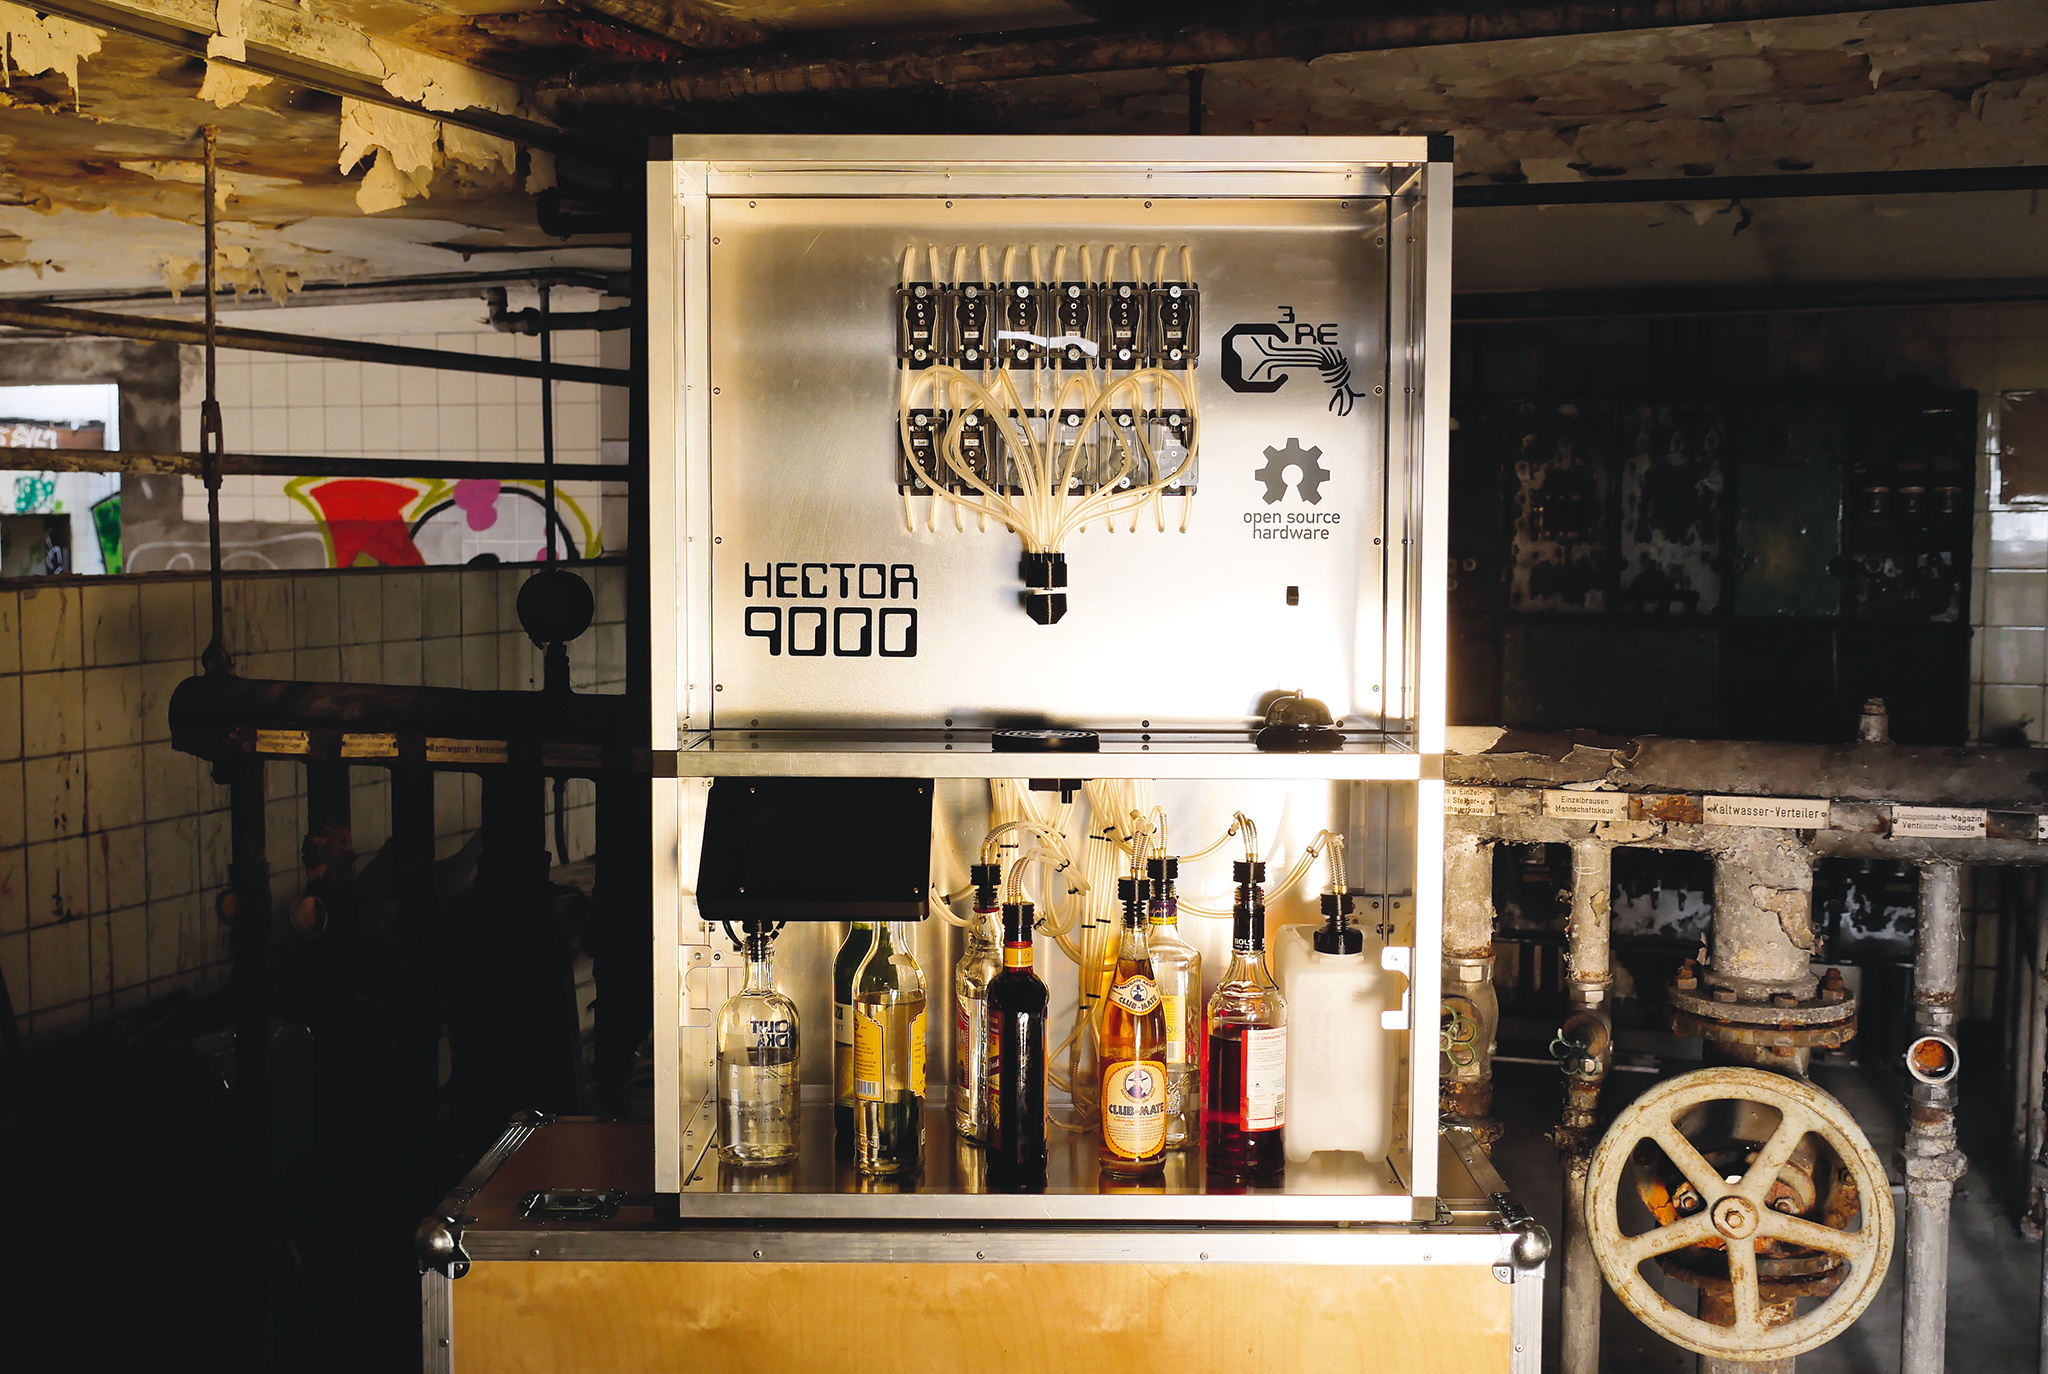
\includegraphics[width=0.7\textwidth]{hector9000.jpg}
	\end{figure}
	
	\newpage
	
	\tableofcontents
	
	\newpage
	
	\section{Einleitung}
		Die Hector 9000 Cocktailmixer-Dokumentation ist eine umfassende technische Anleitung, die alle wichtigen Informationen und Schritte liefert, um den Cocktailmixer erfolgreich in Betrieb zu nehmen. Sie richtet sich an Cocktail-Enthusiasten, Hobbybastler und Technikliebhaber, die ihre eigenen maßgeschneiderten Cocktails zu Hause mixen möchten.
		
		Diese Dokumentation behandelt alle relevanten Aspekte des Projekts. Sie beginnt mit einer detaillierten Erläuterung der Funktionsweise des Hector 9000 Cocktailmixers, gefolgt von klaren Anweisungen zur Anschluss- und Elektroplanung. Es werden ausführliche Informationen zur Hardware des Mixers bereitgestellt, einschließlich der verschiedenen Komponenten und Sensoren, die verwendet werden.
		
		Des Weiteren enthält die Dokumentation präzise Anleitungen zur Montage des Mixers und hilfreiche Tipps, um eine stabile und funktionale Konfiguration zu gewährleisten. Der Installationsprozess der erforderlichen Software wird ebenfalls ausführlich erläutert, einschließlich der Konfigurationsoptionen.
		
		Unser Ziel ist es, Ihnen alle notwendigen Informationen zur Verfügung zu stellen, um den Hector 9000 Cocktailmixer erfolgreich in Betrieb zu nehmen. Wir möchten sicherstellen, dass Sie die erforderlichen Schritte verstehen und umsetzen können, um den Cocktailmixer optimal nutzen zu können.
		
		Diese Dokumentation bietet eine klare und umfassende Anleitung für die erfolgreiche Inbetriebnahme des Hector 9000 Cocktailmixers.
	
	\newpage
	\raggedright
	
	
	
	\section{Materialliste}
	\subsection{Sonstige Teile}
	\begin{tabular}{|l|c|c|r|}
	\hline
	Anzahl & Bezeichnung & Kommentar & Quelle \\
	\hline
	1 & Adafruit PCA9685 Servo Driver	& &	Amazon \\
	\hline	
	1 &	Raspberry Pi 3B	& &	Amazon \\
	\hline
	1 &	PC-Netzteil	 & & Reichelt \\ 
	\hline
	ca. 1.5 m &	LED-Streifen WS2812B	12VDC-Variante! & &	Amazon \\
	\hline
	ca. 30 m	 & Silikonschlauch 6 mm x 4 mm &	lebensmittelecht & Amazon	\\
	\hline	
	1 &	Spültrichter Variante A oder B	& Flush-funnel-XY.stl &	3D-gedruckt \\
	
	\hline
	\end{tabular}
	
	\subsection{Teileliste Arm}
    \begin{tabular}{|l|c|c|r|}
    \hline
        Anzahl & Bezeichnung & Kommentar & Quelle \\ \hline
        1 & Halterung & Arm\_mount.stl & 3D-gedruckt \\ \hline
        1 & Gleiteinsatz & Arm\_sliding\_element.stl & 3D-gedruckt \\ \hline
        1 & Zahnstange & Arm\_rack.stl & 3D-gedruckt \\ \hline
        1 & Ritzel & Arm\_pinion.stl & 3D-gedruckt \\ \hline
        1 & Auslöser & Arm\_trigger.stl & 3D-gedruckt \\ \hline
        1 & Dosierkopf & Arm\_pourer.stl & 3D-gedruckt \\ \hline
        1 & Tropfenfänger & Arm\_drip\_pan.stl & 3D-gedruckt \\ \hline
        1 & Gabellichtschranke & ~ & Amazon \\ \hline
        1 & Pololu A4988 & ~ & Amazon \\ \hline
        1 & NEMA 17 Schrittmotor & ~ & Amazon \\ \hline
        1 & Alu-Vierkantprofil 15.5x15.5 & Länge ist v. Gehäuse abhängig & Baumarkt \\ \hline
        1 & DIN 7981 Blechschraube 2.9x6.5 & ~ & Wegertseder \\ \hline
        4 & ISO 7380 Schraube M3x6 & ~ & Wegertseder \\ \hline
        4 & ISO 7380 Schraube M3x10 & ~ & Wegertseder \\ \hline
        6 & DIN 125 Unterlegscheibe 3.2 & ~ & Wegertseder \\ \hline
        2 & DIN 934 Sechskantmutter M3 & ~ & Wegertseder \\ \hline
        3 & DIN 934 Sechskantmutter M4 & ~ & Wegertseder \\ \hline
        1 & DIN 466 Rändelmutter M4 & ~ & Wegertseder \\ \hline
        6 & DIN 125 Unterlegscheibe 3.2 & ~ & Wegertseder \\ \hline
        2 & Blindnietmutter M3x10 flach & ~ & Wegertseder \\ \hline
    \end{tabular}
    
    \subsection{Teileliste Display}
    \begin{tabular}{|l|l|l|l|}
    \hline
        Anzahl & Bezeichnung & Kommentar & Quelle \\ \hline
        1 & Oberteil & Display\_lid.stl & 3D-gedruckt \\ \hline
        1 & Unterteil & Display\_base.stl & 3D-gedruckt \\ \hline
        1 & Klemme & Display\_clamp.stl & 3D-gedruckt \\ \hline
        1 & Touch-Display 7" & Touch-Funktion über USB! & Amazon \\ \hline
        4 & Distanzbolzen M3 x 10 & männlich-weiblich & Amazon \\ \hline
        2 & Schraube für Thermoplaste 3x10 & ~ & Wegertseder \\ \hline
        4 & ISO 7380 Schraube M3x16 & ~ & Wegertseder \\ \hline
        4 & DIN 934 Sechskantmutter M3 & ~ & Wegertseder \\ \hline
    \end{tabular}
    
    \subsection{Teileliste Glocke}
        \begin{tabular}{|l|l|l|l|}
    \hline
        Anzahl & Bezeichnung & Kommentar & Quelle \\ \hline
        1 & Glockenhalterung & Bell\_base.stl & 3D-gedruckt \\ \hline
        1 & Motorhalterung & Bell\_servo-bracket.stl & 3D-gedruckt \\ \hline
        1 & Finger & Bell\_finger.stl & 3D-gedruckt \\ \hline
        1 & Servo TowerPro MG996R & nur die originalen & HobbyKing \\ \hline
        1 & Tischglocke & ~ & Amazon \\ \hline
        7 & ISO 7380 Schraube M3x10 & ~ & Wegertseder \\ \hline
        7 & ISO 7380 Schraube M3x12 & ~ & Wegertseder \\ \hline
        11 & DIN 934 Sechskantmutter M3 & ~ & Wegertseder \\ \hline
    \end{tabular}
    
    \subsection{Teileliste Pumpe}
    \begin{tabular}{|l|l|l|l|}
    \hline
        Anzahl & Bezeichnung & Kommentar & Quelle \\ \hline
        1 & Sockel & Schego\_830\_mount.stl & 3D-gedruckt \\ \hline
        1 & Membranpumpe Schego 830 &  & Amazon \\ \hline
        2 & Streifen aus Moosgummi 13 mm x 70 mm & & Bastelladen \\ \hline
        2 & U-Profil Aluminium 13 mm x 8 mm x 105 mm & & Baumarkt \\ \hline
        4 & Gewindestange M3x65 & ~ & Baumarkt \\ \hline
        12 & DIN 934 Sechskantmutter M3 & ~ & Wegertseder \\ \hline
    \end{tabular}
    
    \subsection{Teileliste Stopfen}
    
    \begin{tabular}{|l|l|l|l|}
    \hline
        Anzahl & Bezeichnung & Kommentar & Quelle \\ \hline
        12 & Stopfen & Rubberplug\_core.stl & 3D-gedruckt \\ \hline
        12 & Long-Life Corky 0.7 l-1.0 l & ~ & METRO \\ \hline
    \end{tabular}
	
	
	\subsection{Teileliste Ventile}
	    \begin{tabular}{|l|l|l|l|}
    \hline
        Anzahl & Bezeichnung & Kommentar & Quelle \\ \hline
        12 & Ventilgehäuse & Valve\_body.stl & 3D-gedruckt \\ \hline
        12 & Nocken & Valve\_cam.stl & 3D-gedruckt \\ \hline
        24 & Zunge & Valve\_tongue.stl & 3D-gedruckt \\ \hline
        12 & Deckel PMMA & Valve\_cover.stl & CNC/Laser \\ \hline
        12 & TowerPro MG996R Servo & nur die originalen & Hobbyking \\ \hline
        24 & DIN 965 Schraube M3x8 & ~ & Wegertseder \\ \hline
        48 & ISO 7380 Schraube M3x10 & ~ & Wegertseder \\ \hline
        24 & DIN 933 Schraube M3x35 & ~ & Wegertseder \\ \hline
        72 & DIN 934 Sechskantmutter M3 & ~ & Wegertseder \\ \hline
        24 & DIN 466 Rändelmutter M3 & ~ & Wegertseder \\ \hline
    \end{tabular}
    
    \subsection{Teileliste Waage}
        \begin{tabular}{|l|l|l|l|}
    \hline
        Anzahl & Bezeichnung & Kommentar & Quelle \\ \hline
        1 & Überlaufgitter & Scale\_overflow\_grid.stl & 3D-gedruckt \\ \hline
        1 & Überlaufrohr & Scale\_overflow\_pipe.stl & 3D-gedruckt \\ \hline
        1 & Waagschale & Scale\_pan.stl & 3D-gedruckt \\ \hline
        1 & Abstandshalter & Scale\_spacer.stl & 3D-gedruckt \\ \hline
        1 & Gehäuse & Scale\_cover.stl & 3D-gedruckt \\ \hline
        1 & Deckel & Scale\_lid.stl & 3D-gedruckt \\ \hline
        1 & Kabelverschraubung M10 & ~ & eBay \\ \hline
        4 & Schraube für Thermoplaste 3x10 & ~ & Wegertseder \\ \hline
        1 & Wägezelle 1 kg mit HX711-Board & ~ & Amazon \\ \hline
    \end{tabular}
	

	
	\begin{figure}
	\section{Hector 9000 Aufbau}
	\subsection{Frontansicht}
	\begin{center}
	\includegraphics[scale=0.5]{"hector9000-vorne.jpeg"}	
	\end{center}


	\subsection{Hinterseite}
	\begin{center}
	\includegraphics[scale=0.5]{"hector9000-hinten.jpeg"}		
	\end{center}
	\end{figure}
	
	
	\newpage
	\section{Hardware}
	
	
	\begin{lstlisting}[language=bash]


	\end{lstlisting}
	
\end{document}
